\chapter{Prescription for fragment identification via localization function}\label{append:Fragments}
As mentioned in Section~\ref{sect:FragID}, we have developed a method for estimating primary fission yields using the nucleon localization function and a PES which has been computed out to the outer turning line. In fact, a 1D PES might be sufficient for some purposes, while still giving a distribution which is plausible.

Our prescription is the following:

\begin{itemize}
	\item Identify possible prefragments using the density and nucleon localization function (see Figure~\ref{fig:methods240Pulocali}):
	\subitem Along the primary axis of the nucleus, find the two locations (one for each fragment) at which the density is widest. This is taken to be the approximate center of each fragment.
	\subitem For each fragment, start from the central value and locate the two nearest optima in the localization (maximum or minimum; one on either side). This gives you a range of possible central values.
	\subitem Sum up the nucleons above (below) the central value and multiply by two to determine the identity of the upper (lower) prefragment.
	\item The remaining neck nucleons are assumed to form into clusters: alpha particles first, then a deuteron if there is one of each nucleon left, plus some remaining free protons or neutrons.
	\item The total binding energy of the prefragments and any particles/clusters is subtracted from the total energy of the system to get the energy of the neck, $E_{neck}$.
	\subitem Use this energy to define the temperature of the system: $T = \sqrt{\left|E_{neck}/a\right|}$ where the level density parameter $a$ we take to be $a=A_p/10$ MeV$^{-1}$ with $A_p$ the mass number of the parent nucleus.
	\item Use brute force combinatorics to find every possible way of assigning the neck particles to either of the prefragments (including the possibility that a particle/cluster might be emitted instead of flowing to a prefragment).
	\item For each fragments + particles combination, look up the binding energy of each of the final fragments in a table (such as  MassExplorer \cite{massexplorer}).
	\item The Coulomb repulsion energy between the fragments plus the total binding energy of the fragments and any remaining clusters is subtracted from the total energy of the system to get the residual (kinetic + intrinsic) energy, $E_{res}$.
	\item I use this energy to define the a grand canonical ensemble (note that the chemical potentials are hidden in the binding energies): $Z = \sum e^{-\frac{E_{res}}{k_BT}}$
	\item Calculate probabilities: $P(n_1,z_1,n_2,z_2) = \frac{1}{Z} e^{-\frac{E_{res}(n_1,z_1,n_2,z_2)}{k_BT}}$
	\item Fold those probabilities with a Gaussian smoothing function.
\end{itemize}

\begin{figure}
	\centering
	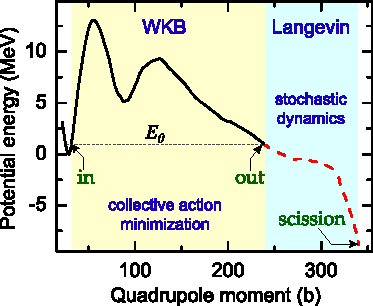
\includegraphics[width=0.5\linewidth]{TeX_files/methods_overview}
	\caption[Localization function for 240Pu with lines drawn to represent prefragment identification]{Localization function for 240Pu with lines drawn to represent prefragment identification}
	\label{fig:methods240Pulocali}
\end{figure}

The fact that this can be estimated at the outer turning line instead of at scission is a tremendous reduction in the number of PES points which must be computed. Furthermore, our experience with the WKB approximation shows that most trajectories leading to the outer turning line actually follow the minimum action path, branching away only just before reaching the outer turning line. In Chapter~\ref{chap:rprocess}, we will compute a 1-dimensional PES between the ground state and the outer turning line (either the static path or the minimum action path), and a 2-dimensional PES in the region of the outer turning line. This is a substantial reduction compared to the Langevin calculations, but the $^{240}$Pu SF yields shown in Figure~\ref{fig:methods240Puyield} are similar, with similar peaks and widths, but with appropriately wider uncertainty bands for the localization + grand canonical ensemble method.

\begin{figure}
	\centering
	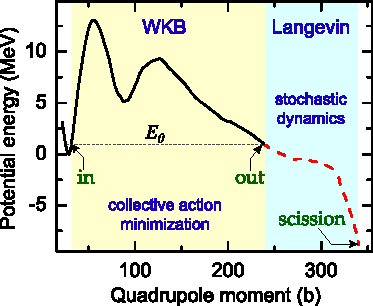
\includegraphics[width=0.5\linewidth]{TeX_files/methods_overview}
	\caption[Computed spontaneous fission yields for 240Pu compared to experimental data. The Langevin yields are shown in ??? color and are taken from~\cite{Sadhukhan2016}. The localization yields are shown in ??? color. Experimental data is shown in ??? color and comes from ??? source.]{Computed spontaneous fission yields for 240Pu compared to experimental data. The Langevin yields are shown in ??? color and are taken from~\cite{Sadhukhan2016}. The localization yields are shown in ??? color. Experimental data is shown in ??? color and comes from ??? source.}
	\label{fig:methods240Puyield}
\end{figure}

We should also show {\Og} calculations here, and perhaps even {\Pt} calculations too, if you can get them in time.

%\section{The problem of scission}
%For practical reasons discussed in Chapter~\ref{chap:Model}, we are limited to describing complicated shapes in terms of just a few parameters, leading to uncertainty in the properties of the fragment. In particular, the part of the process at which the neck snaps and one nucleus becomes two, called scission, is not well-defined in static approaches.
%
%Many times in static approaches, including most of the results shown in this dissertation, scission is characterized by a single number such as $q_N$, which corresponds to the size of the neck. When that number falls below a certain predefined threshold, we say that the nucleus has scissioned. Fragments are identified and one can try to estimate the strength of the repulsive interaction forcing the fragments apart. Of course, as discussed in~\cite{Bonneau2007,Younes2011}, wavefunctions corresponding to individual nucleons may have tails which extend into the opposite fragment. This is especially problematic for estimating energies and other observables beyond the mass and charge.
%
%This can be understood with an analogy: suppose we stretch a nucleus until a neck forms, and then we use a butcher knife to lop the two fragments apart. This works reasonably well for estimating fragment mass and charge, but it does very poor job of estimating the relative energy of the fragments. To estimate fragment kinetic and excitation energies, one needs to carefully and delicately peel the interlocking fragments apart with a scalpel, or a proper accounting of entanglement and other many-body correlations.
%
%
%\section{Fragments and the nucleon localization function}
%An improved scission criterion would go beyond simply counting the number of particles in the neck. To help with this, we have a tool at our disposal which helps us to understand correlations that affect fission dynamics. This is called the nucleon localization function, and it allows us to visualize the prefragment nuclear shell structure which largely determines the identity of fission fragments~\cite{Zhang2016}.
%
%The nucleon localization function shows that some prefragments can be very well-formed even when the neck is large, while in another case the neck might be small but the prefragments poorly-defined (compare Figures~\ref{fig:178ptunedf1pes} and~\ref{fig:294oglocali}). A better scission criterion should take into account, or be compatible with, the insights gained from the nucleon localization function. As noted in~\cite{Younes2009}, fragment properties on either side of the scission line may differ drastically. This is because shell structure is not well-described by multipole moments of the density. The localization measure offers an alternative method for identifying fragments before the scission line (see~\cite{Sadhukhan2017}). Since it is based on the underlying quantum shells, it is less sensitive to fluctuations and particle rearrangements late in the evolution.
%
%

%\section{Prefragment shell structure}
%A common theme in all of this has been the importance of the underlying shell structure of the prefragments. Shell energy corrections were found to be important in {\Pt} and {\Hg}; cluster formation in {\Og} was clearly influenced by the shell structure of the fragments; and the same may or may not be the case for {\Cf}. Let's discuss this.
%
%We used localizations to visualize the internal/intrinsic shell structure inside nuclei, and we were able to see that this structure was sometimes intact early in the evolution, at times as far back as the outer turning line. And actually, this kind of makes sense. From just energetics alone, a nucleus on the outer turning line is just as happy (or just as stable, or just as settled) as a nucleus in the ground state. In some sense, it is formed. The difference now is just that the configuration it's in is now unstable due to Coulomb. The two halves, which are kind of maybe happy from a nuclear physics perspective, are pushing apart from the Coulomb repulsion. So that still has to be carried out, but the bulk of the physics might already be done at this point - though not necessarily. It \textit{could} be that the fragments are well-formed and just pushing apart, but that may not be the case. It's like a divorce: sometimes the two have drifted so far apart, or are so well-defined and incompatible as individuals that the divorce is simple and relatively straightforward. Other times, it is a mess trying to sort out who gets what, and the two parties are fundamentally-changed by the proceedings.
%
%I don't have any strong objections to Scamps and Simenel's octupole paper. In fact, to me it kind of makes sense: we've been saying, after all, that it's the shell structure of the deformed prefragments which determine scission, and not necessarily the final fragments themselves. That's really the whole idea behind the localization paper: we're seeing that, at least in some cases, the shell structure is pretty well intact early in the evolution, and that those prefragments drive the system to scission with some shuffling of the neck nucleons at scission. All they're saying is that those neck nucleons will affect the shell structure of the prefragments, and just based on the kinds of shapes that the system will take (small neck connecting two elongated or spherical fragments), the prefragments have a strong octupole moment (regardless of whether the fragments are elongated or spherical). So it shouldn't be the spherical magic numbers we worry about, but the deformed (in this case, octupole-deformed) magic numbers.
%
%I feel like it shouldn't be too terrible to investigate this claim. What if we constrained the multipole moment(s) that correspond(s) to octupole-deformed fragments (perhaps $Q_{50}$)? I think this parameter might be included in Peter Moller's model, but not in ours.
%
%
%\section{Isospin transport}
%We're assuming that the parent nucleus gets to however it gets at the OTL (maybe it just happens to oscillate into that configuration randomly one day, and it feels reasonably stable there (per Witek's deformed harmonic oscillator paper)), and now we're trying to argue about how the neck nucleons will flow to rearrange themselves. So we're already imposing the assumption that the nucleons \textit{will} flow from the neck to the fragments (and indeed, that at least seems to be what happens based on the success of this type of model so far).
%
%This is indeed in contradiction with Scamps and Simenel's paper, because they essentially claim that once you get to that OTL configuration, the octupole deformation of the fragments (created by a spherical-ish prefragment with neck nucleons on the side, giving it a non-zero Q30) is sufficiently strong to snap the neck and let the fragments go on their merry way, octupole-deformed and everything. On the other hand, we're saying that instead, it's just a lucky coincidence that the fragments are stable in an octupole-deformed configuration because they're not going to stay that way once the neck nucleons flow to their final destination.
%
%There are these isospin transport papers essentially describe the flow of isospin and density in terms of the chemical potential and gradients. Nucleons will flow based on the chemical potential* properties of the system, or in other words, to minimize the binding energy of the system. In general, that means you'll see a flow of neck nucleons in such a way as to bring the final fragments as [jointly] close to stability as possible.
%
%* Reminder on chemical potential: $\mu \equiv \left(\frac{\partial U}{\partial N}\right)_{S,V}$, or essentially the energy per particle which is added/removed from the system. $\mu$ must be negative for bosons (else the grand canonical potential will be an exponentially-increasing function), but it can be positive or negative for fermions
%
%The density gradient terms will lead to a flow of nucleons from prefragments to neck (with apparently a greater effect on neutrons than on protons).
%
%Jhilam sent a couple of experimental papers where alpha clusters were observed emitting from the neck (perpendicular to the momenta of the fragments). Might this localization tool be used to later help model neutron and alpha emission?